\documentclass{beamer}
\setcounter{tocdepth}{1}
\mode<presentation>
{
  \usetheme{Warsaw}
  \setbeamercovered{transparent}
}

\usepackage[english]{babel}
\usepackage{times}
\usepackage{listings}
\usepackage{amsmath,multicol}
\usepackage{verbatim}
\usepackage{beamerarticle}
\usepackage{longtable}
%\usepackage{ucs}
\usepackage[utf8]{inputenc}
\usepackage{pdfpages}
\usepackage{listings}

\usepackage{hyperref}


\AtBeginSection[]
{
  \begin{frame}<beamer>
     \setcounter{tocdepth}{2}
     \tableofcontents[currentsection,currentsubsection,hideothersubsections]
  \end{frame}
}

\addtobeamertemplate{footline}{\insertframenumber/\inserttotalframenumber}



\title{Les solutions de montage vidéo sous Linux}
\date{\today}
\author{Rémi LEBLOND}
\institute{Photo-Ciné-Club d'Alsace}

\begin{document}

\frame[plain]{\titlepage
\begin{center}
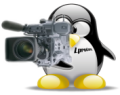
\includegraphics[scale=0.5]{ressources/logo.png}
\end{center}
}

\begin{frame}
 \frametitle{Plan}
 
 \tableofcontents
\end{frame} 

\section{Acquisition vidéo}
\begin{frame}
 \frametitle{Outils d'acquisition vidéo}
\begin{itemize}
\item But : 
\begin{itemize}
\item Récupérer les fichiers vidéo à partir de la caméra
\item Format DV ou HDV
 \end{itemize}
 
 \item Utilisation de l'interface IEE1394 (Firewire ou iLink)
 \end{itemize}
 \begin{itemize}
 \item [dvgrab] Outil en ligne de commande.
 \item [Kino] Outil convivial et efficace.
 \end{itemize}
\end{frame}

\subsection{dvgrab}
\begin{frame}
\frametitle{dvgrab : outil en ligne de commande}
\begin{itemize}
\item Logiciel à tout faire
\item Ligne de commande :
\begin{itemize}
\item Pas très convivial
\item Très puissant
\end{itemize}
\item Souvent utilisé "derrière" une interface graphique plus conviviale
\end{itemize}
\end{frame}

\begin{frame}
\frametitle{Utilisation de dvgrab}
\lstset{language=bash, frame=shadowbox, rulesepcolor=\color{blue}, breaklines=true, breakatwhitespace=true}
\begin{itemize}
\item Capture DV :
\lstinputlisting{ressources/ex_capture_dv.sh}
Mise en lecture du camescope et enregistrement des flux vidéo au format DV et son au format WAV dans un fichier "exemple.avi". 

\item Capture DVHD :
\lstinputlisting{ressources/ex_capture_hdv.sh}
\end{itemize}
\end{frame}

\begin{frame}
\frametitle{Utilisation avancée de dvgrab}
dvgrab dispose de nombreuses options :
\begin{tabular}{|c|p{8cm}|}
\hline
--autosplit & découpe le fichier de capture dès qu'un stop camera est détecté (découpage de scène) \\
\hline
--timestamp & ajoute la date à la fin du radical du nom de fichier donné\\
\hline
-i & lance une capture interactive en ligne de commande qui permet de controler la camera au clavier (appuyez sur « ? » ensuite pour avoir les commandes de contrôles). \\
\hline
 \end{tabular}
 \end{frame}
 
 \subsection{Kino}
 \begin{frame}
 \frametitle{Capture interactive avec Kino}
 \begin{itemize}
 \item Kino : 
  \begin{itemize}
 \item Logiciel libre de capture et d'édition vidéo numérique non linéaire grand public.
 \item Module d'acquisition très performant et simple d'utilisation.
 \end{itemize}
 
 \item Habillage d'outils existants
  \begin{itemize}
 \item \textit{ffmpeg, mencoder et ffmpeg2theora}
 \item \textit{support de la capture 1394 avec dvgrab)}
 \end{itemize} \end{itemize}
 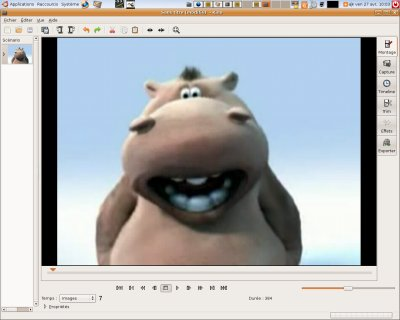
\includegraphics[scale=0.25]{ressources/ecran_kino.jpg}
 \end{frame}
 
 \begin{frame}
 \frametitle{Capture DV avec Kino}
  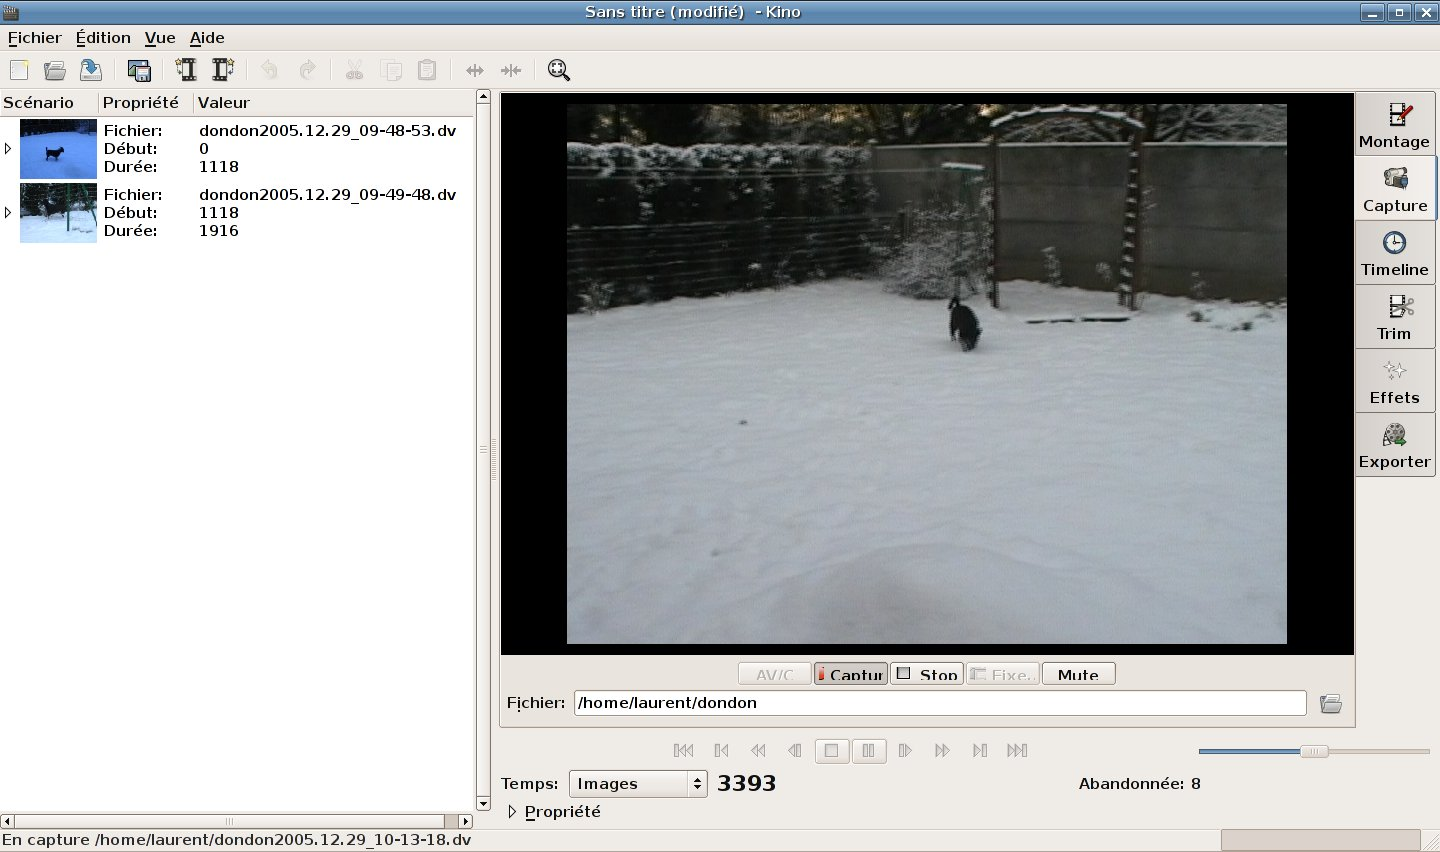
\includegraphics[scale=0.20]{ressources/capture_kino.jpg}
 \end{frame}
 
 \subsection{Autres formats}
 \begin{frame}
 \frametitle{Autres formats vidéo}
Sortie d'appareil photo ou récupération de sources variées :
  \begin{itemize}
 \item AVI, MOV, MPEG...
 \item Motion JPEG
 \end{itemize}
 Conversion préalable au format DV
   \begin{itemize}
 \item Format universellement reconnu (pivot)
 \item Format sans perte
 \item Attention à la taille (vidéo HD)
 \end{itemize}
 $\rightarrow$ Logiciel de transcodage
 \end{frame}

\section{Montage}
\begin{frame}
 \frametitle{Outils de montage les plus courants}
 \begin{itemize}
 \item \textbf{Kino} : outil "tout en un", de l'acquisition au rendu final.
 
 Equivalent à Windows Movie Maker.
 
 Limité fonctionnellement (une seule piste, effets limités...), mais simple et très stable.
 
 \item \textbf{OpenShot Video Editor} clone de Windows Movie Maker ou iMovie. Logiciel récent, mais gros potentiel.
 
 \item \textbf{VLMC} logiciel de montage vidéo issu de l'équipe VLC (lecteur multimédia très réputé).
 
 \item \textbf{Cinelerra} : très puissant et complet, le plus abouti actuellement en logiciel libre. Comparable à Adobe Premiere.
 \end{itemize}

\end{frame}

\subsection{Kino}
\begin{frame}
 \frametitle{Kino}
   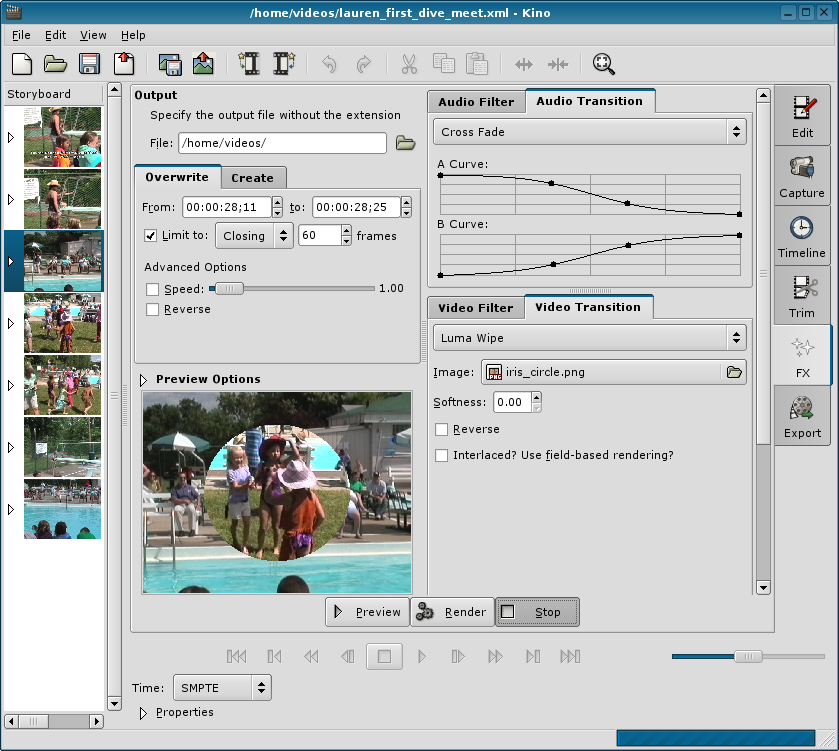
\includegraphics[scale=0.25]{ressources/kino-fx.png}

\end{frame}

\subsection{OpenShot Video Editor}
\begin{frame}
 \frametitle{OpenShot Video Editor}
  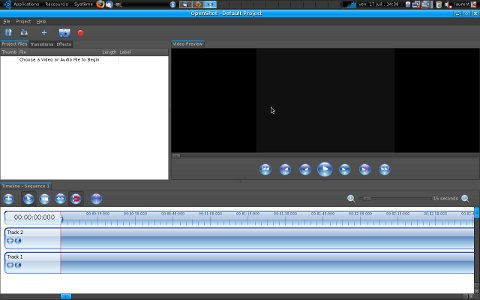
\includegraphics[scale=0.60]{ressources/openshotvideo.jpg}

\end{frame}

\subsection{VLMC}
\begin{frame}
 \frametitle{VLMC}
  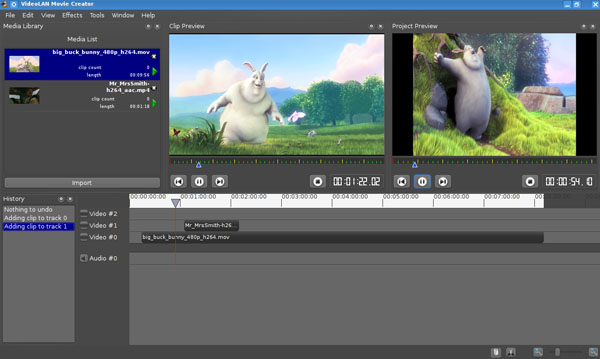
\includegraphics[scale=0.60]{ressources/vlmc.jpg}
\end{frame}

\subsection{Cinelerra}
\begin{frame}
 \frametitle{Cinelerra : Outil de montage "pro"}
  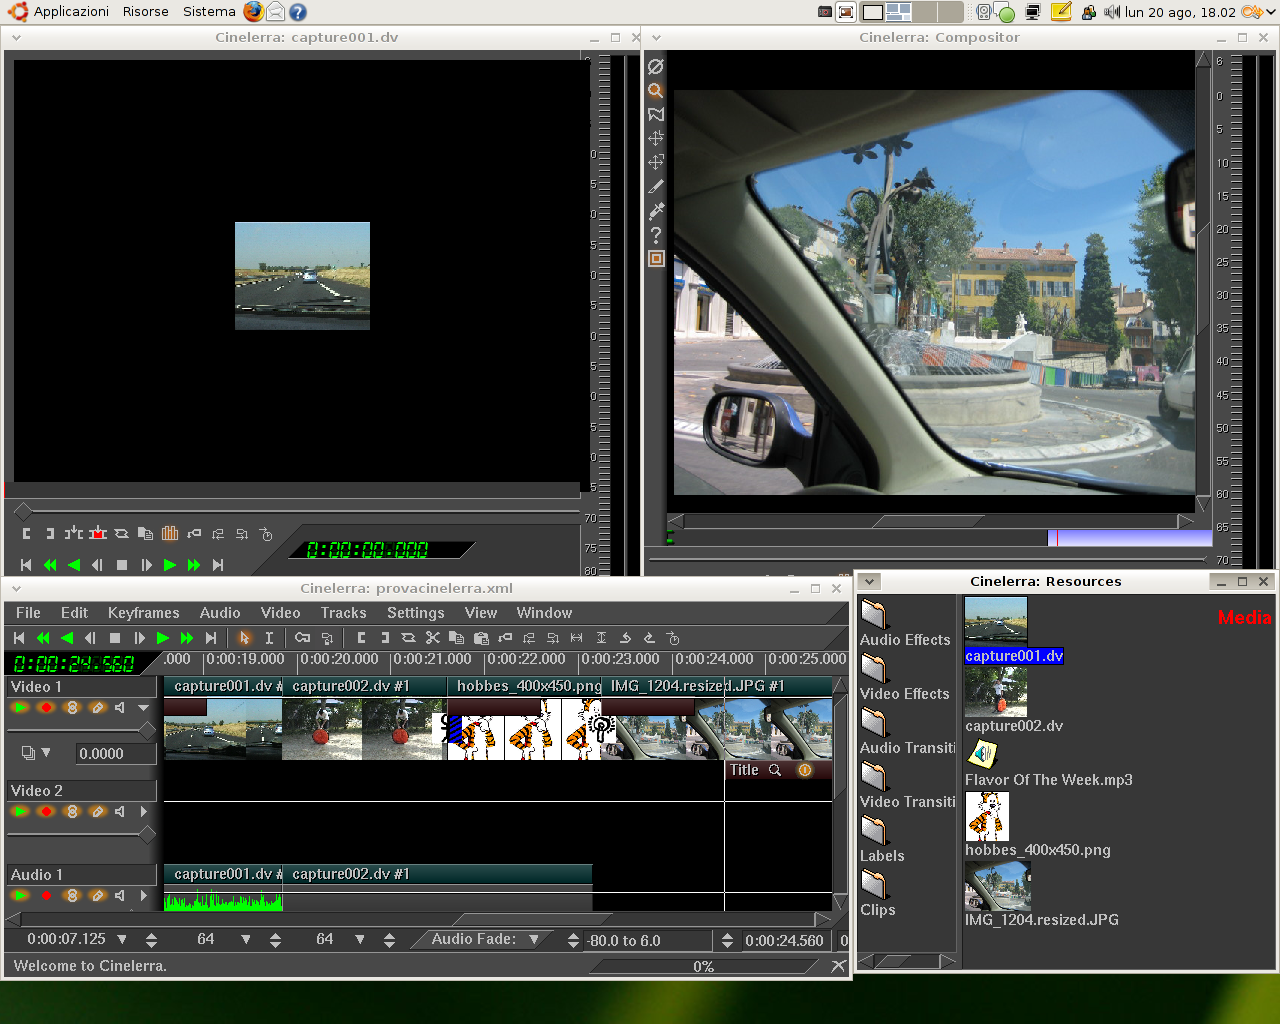
\includegraphics[scale=0.20]{ressources/cinelerra.png}
\end{frame}

\begin{frame}
 \frametitle{Cinelerra : Camera et projecteur virtuels}
 
  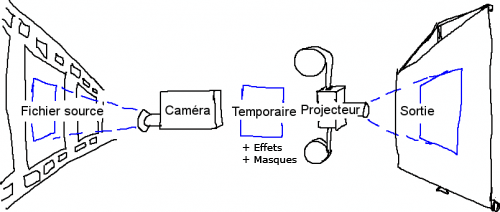
\includegraphics[scale=0.60]{ressources/cinelerra_camera_projecteur.png}
  
  Source : \href{http://www.post-pro.fr/tutos/cinelerra/}{http://www.post-pro.fr/tutos/cinelerra/}
\end{frame}

\begin{frame}
 \frametitle{Cinelerra : Images clefs}
 \begin{itemize}
 \item Courbes
 \item Permettent de faire varier la plupart des paramètres
 \end{itemize}
  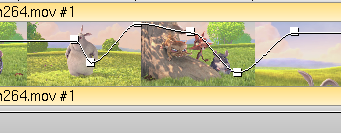
\includegraphics[scale=1]{ressources/cinelerra-image-clef.png}
  
  Source : \href{http://www.post-pro.fr/tutos/cinelerra/}{http://www.post-pro.fr/tutos/cinelerra/}
\end{frame}


\section{Post-production vidéo}
\begin{frame}
 \frametitle{Post-production vidéo}
  
  \begin{itemize}
\item \textbf{Jahshaka} : Composition, montage vidéo avancé, effets spéciaux et post-production comparable au logiciel de référence propriétaire Adobe After effects. 

Le projet s'appele désormais Cinefx depuis début 2008.

 \item \textbf{CinePaint} : Outil de retouche d'image dérivé de Gimp et spécialisé dans la retouche d'image animées (flipbook).
\item \textbf{Manslide} : Création de diaporama vidéo à partir d'images fixes.
\item \textbf{Stopmotion} : Création d'animation vidéo, de dessin animés à partir d'image fixe légèrement décalée en utilisant la technique du stop motion.
\item \textbf{Pencil}, 	\textbf{Synfigstudio} : Outils d'animation 2D.
 \end{itemize}
\end{frame}

\subsection{Jahshaka}
\begin{frame}
\frametitle{Jahshaka : puissant outil de post-production}
Site officiel Cinefx, alias jahshaka : \href{http://www.cinefx.org/}{http://www.cinefx.org/}

\href{http://download.tuxfamily.org/lprod/tutoriels/tutoriel_jahshaka_niv1_debutant.pdf}{Tutoriel rapide en ligne}.
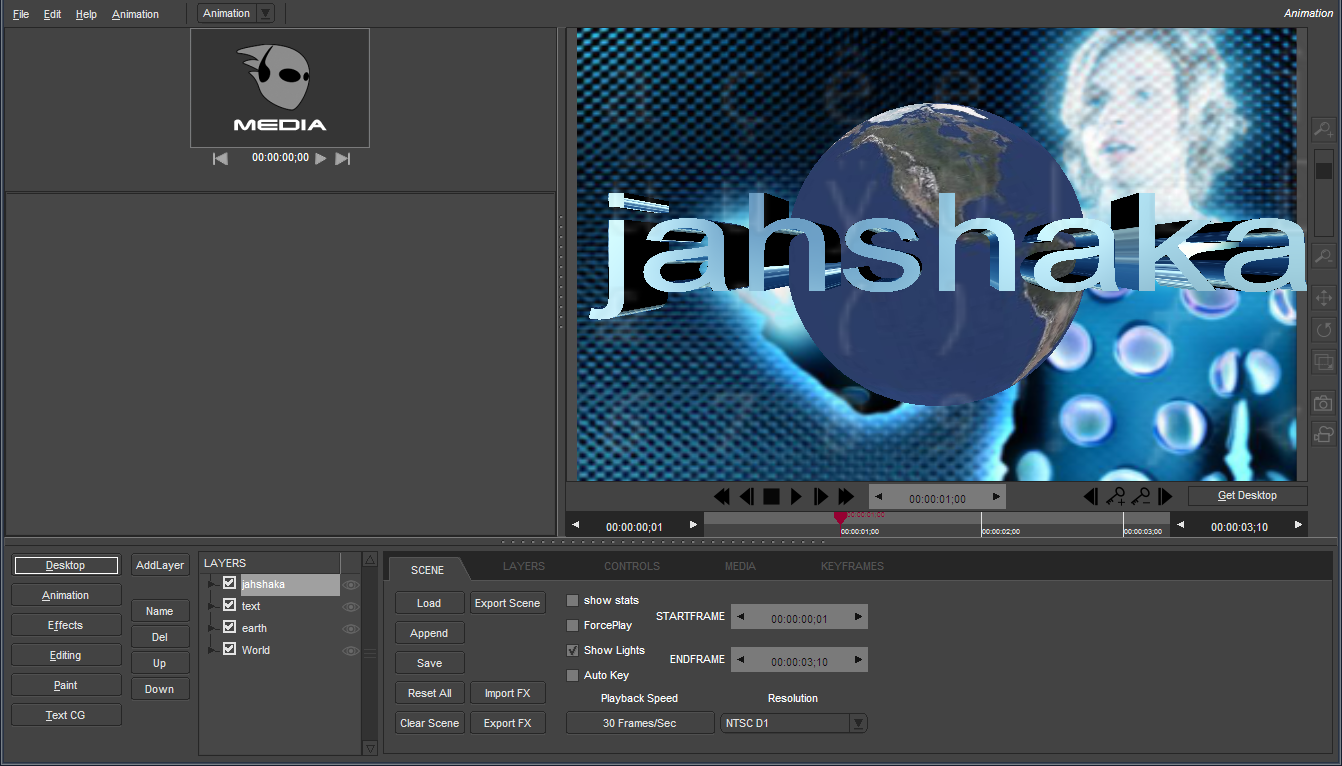
\includegraphics[scale=0.20]{ressources/jahshaka.png}
\end{frame}

\subsection{CinéPaint}
\begin{frame}
\frametitle{CinéPaint : outil de retouche d'images}
\begin{itemize}
\item Dérivé de "The Gimp"
\item Spécialisé dans la retouche d'images animées (flipbook)
\item Support des images 8, 16 et 32 bits
\end{itemize}

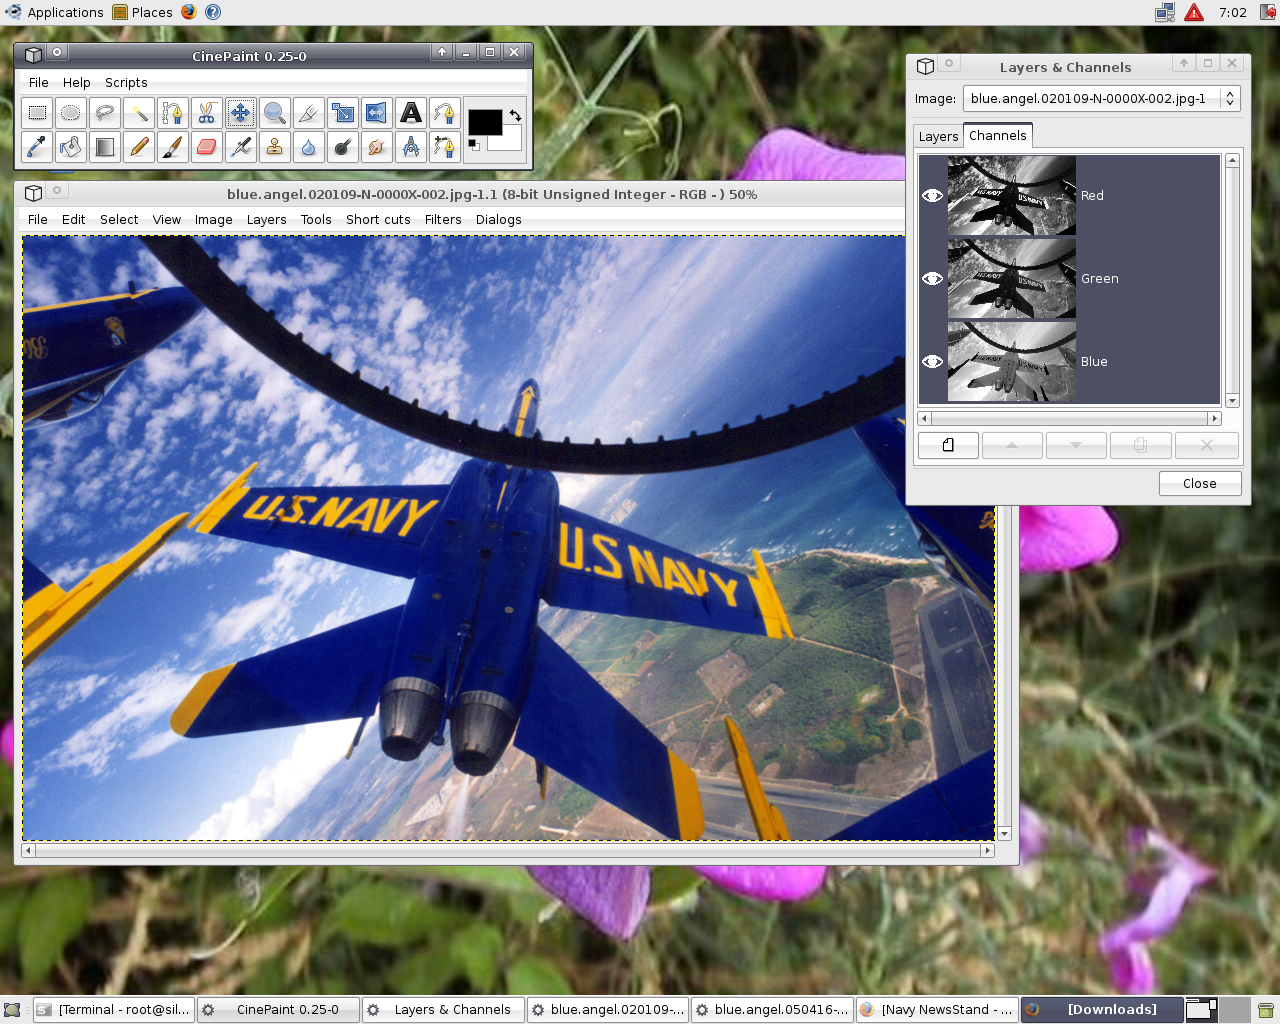
\includegraphics[scale=0.15]{ressources/cinepaint.png}
\end{frame}

\subsection{Avidemux}
\begin{frame}
\frametitle{Avidemux : Editeur vidéo}
\begin{itemize}
\item Permet d'effectuer des coupes, d'appliquer des filtres et de réencoder des vidéos
\item Equivalent de VirtualDub
\item Peut être utilisé pour extraire des images fixes d'une vidéo (pour retouche CinéPaint, par exemple)
\end{itemize}
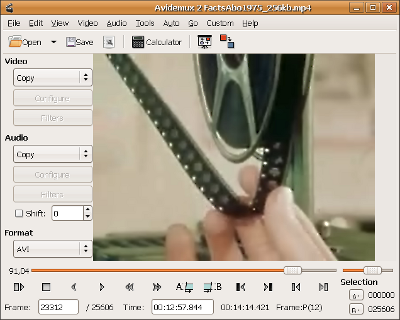
\includegraphics[scale=0.3]{ressources/avidemux.png}

\end{frame}

\subsection{Pencil}
\begin{frame}
\frametitle{Pencil : outil d'animation vectorielle}
Site officiel du logiciel : \href{http://pencil-animation.org/wiki/doku.php?id=en:users:manual:0.4.3b:index}{http://pencil-animation.org}
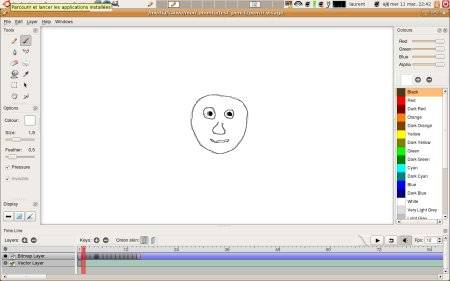
\includegraphics[scale=0.50]{ressources/pencil.jpg}
\end{frame}

\subsection{Synfigstudio}
\begin{frame}
\frametitle{Synfigstudio : puissant outil d'animation vectorielle}
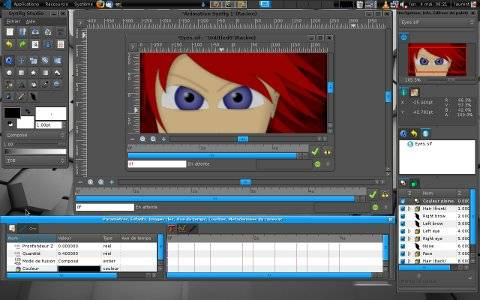
\includegraphics[scale=0.50]{ressources/Synfigstudio.jpg}
\end{frame}

\section{Traitement du son}
\subsection{Audacity}
\begin{frame}
 \frametitle{Audacity : outil de traitement du son}
 \begin{itemize}
\item Logiciel libre d'édition musicale et de montage audio.
\item Complet et très simple, c'est le couteau suisse de la musique libre.
\item Logiciel multi-plateforme (Linux, Windows et MacOsX).
\end{itemize}
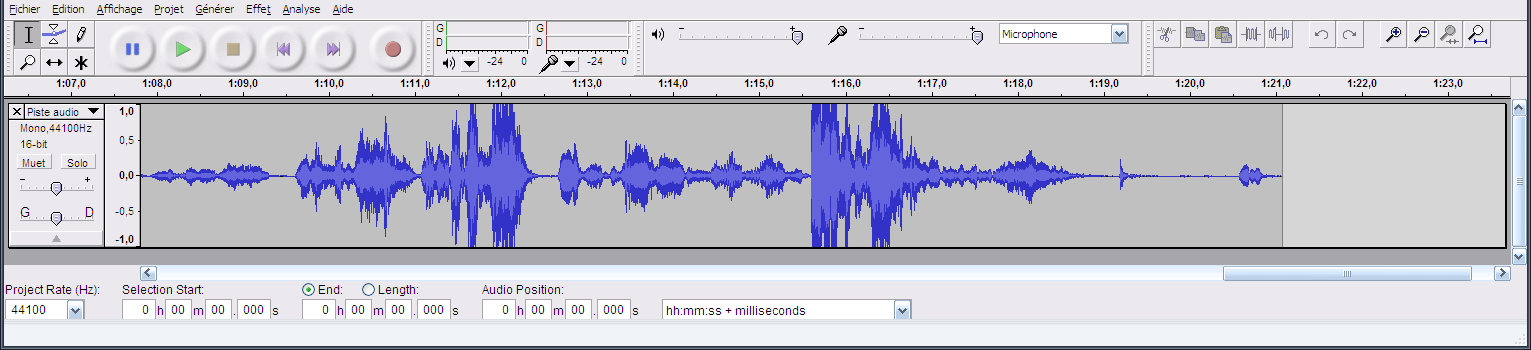
\includegraphics[scale=0.22]{ressources/audacity.png}
\end{frame}

\subsection{Soutitrage}
\begin{frame}
 \frametitle{Soutitrage}
 Création de fichier SRT.
 
 Outils disponibles :
 \begin{itemize}
\item KSubtile : \href{http://ksubtile.sourceforge.net/}{http://ksubtile.sourceforge.net/}
\item Gaupol : \href{http://home.gna.org/gaupol/}{http://home.gna.org/gaupol/}
\item Jubler : \href{http://www.jubler.org/}{http://www.jubler.org/}
\end{itemize}
\end{frame}

\begin{frame}
 \frametitle{Soutitrage avec KSubtile}
 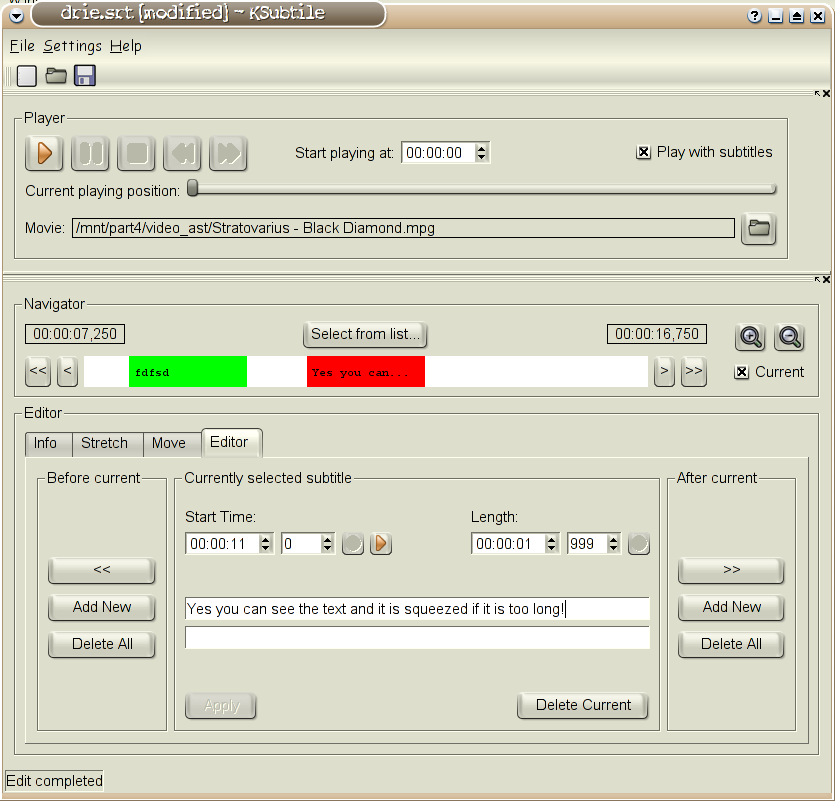
\includegraphics[scale=0.25]{ressources/ksubtile.png}
 \end{frame}
 
\begin{frame}
 \frametitle{Soutitrage avec Jubler}
 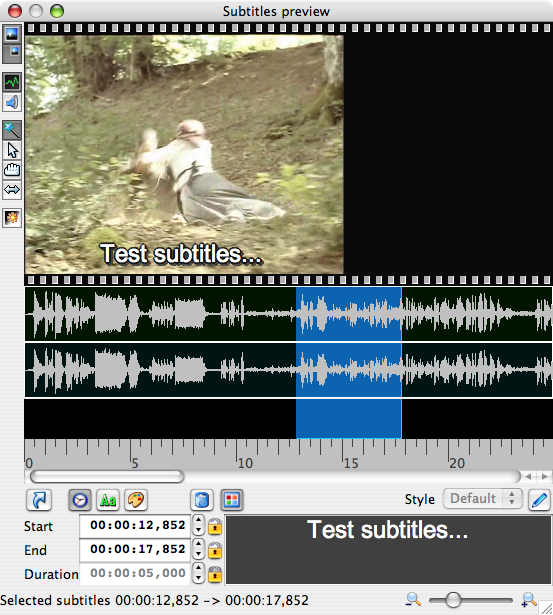
\includegraphics[scale=0.30]{ressources/jubler.jpg}
 \end{frame} 

\begin{frame}
 \frametitle{Soutitrage avec Gaupol}
 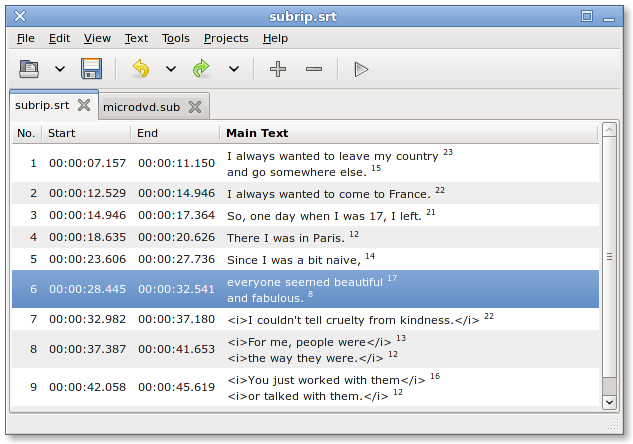
\includegraphics[scale=0.35]{ressources/gaupol.png}
 \end{frame}

\section{Encodage et autoring}
\subsection{Mencoder}
\begin{frame}
\frametitle{\textbf{mencoder} : encodage en ligne de commande}

\begin{itemize}
\item Le couteau suisse de l'encodage vidéo.
\item "Petit frère" du logiciel Mplayer.
\item Très nombreux formats supportés

(en lecture et en écriture).
\item Utilisable en ligne de commande
\item Interface graphique : \textit{ressources/gmencoder}
\end{itemize}
\end{frame}

\begin{frame}
\frametitle{\textbf{mencoder} : encodage en ligne de commande}

\lstset{language=bash, frame=shadowbox, rulesepcolor=\color{blue}, breaklines=true, breakatwhitespace=true}
\begin{itemize}
\item Encoder en DV 4/3 : 
\lstinputlisting{ressources/ex_encode_dv43.sh}

\item Encoder en DV 16/9 : 
\lstinputlisting{ressources/ex_encode_dv169.sh}
\end{itemize}
\end{frame}

\begin{frame}
\frametitle{\textbf{mencoder} : encodage en ligne de commande}
\lstset{language=bash, frame=shadowbox, rulesepcolor=\color{blue}, breaklines=true, breakatwhitespace=true}
\begin{itemize}
\item Encoder en AVI/Mpeg4 :
\lstinputlisting{ressources/ex_encode_mp4.sh}

\item Encodage en flash vidéo pour le web :
\lstinputlisting{ressources/ex_encode_flash.sh}
\end{itemize}
\end{frame}

\begin{frame}
\frametitle{\textbf{mencoder} : encodage en ligne de commande}
\lstset{language=bash, frame=shadowbox, rulesepcolor=\color{blue}, breaklines=true, breakatwhitespace=true}
\begin{itemize}
\item Transformer un fichier vidéo WMV en AVI :
\lstinputlisting{ressources/ex_transfo_wmv2avi.sh}

\item Intégration de sous-titre :
\lstinputlisting{ressources/ex_int_stitre.sh}
\end{itemize}
\end{frame}

\subsection{gMencoder}
\begin{frame}
\frametitle{gmencoder : exemple de fenêtre}
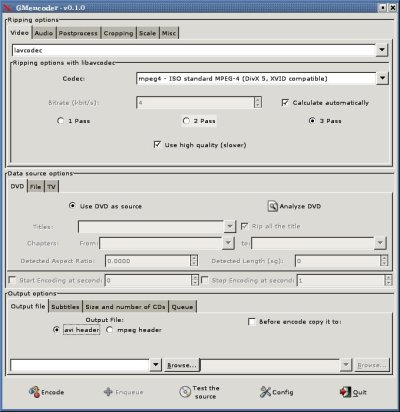
\includegraphics[scale=0.40]{ressources/gmencoder.jpg}
\end{frame}

\subsection{EKD}
\begin{frame}
\frametitle{EKD : EnKoDeur}
\begin{itemize}
\item Opérations de post-production sur vidéos/son/images
\item Site Web : \href{http://ekd.tuxfamily.org}{http://ekd.tuxfamily.org}
\item Fonctions :
\begin{itemize}
\item Gestion des vidéos
\begin{itemize}
\item Transcodage dans différents formats
\item Montage très simple
\item Découpage/redimentionnement
\item Conversion en images fixes / création de diaporama
\item Modification de la fréquence d'images
\end{itemize}
\item Gestion des images
\begin{itemize}
\item Module de compositing (assemblage de scènes)
\item Transition d'images
\item Masques (découpage, couche alpha... )
\item Filtres d'effet (bande dessinée, sépia, renforcement, flou... )
\end{itemize}
\item Gestion des fichiers audio
\end{itemize}
\end{itemize}
\end{frame}


\begin{frame}
\frametitle{EKD : Transcodage}
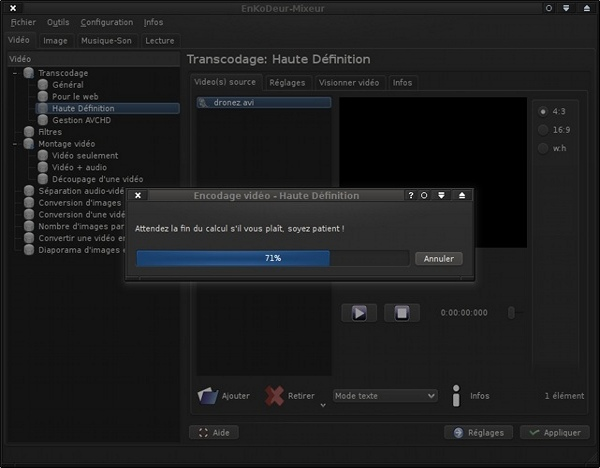
\includegraphics[scale=0.50]{ressources/ekd_linux_transcode.jpg}
\end{frame}

\begin{frame}
\frametitle{EKD : Redimentionnement de vidéo}
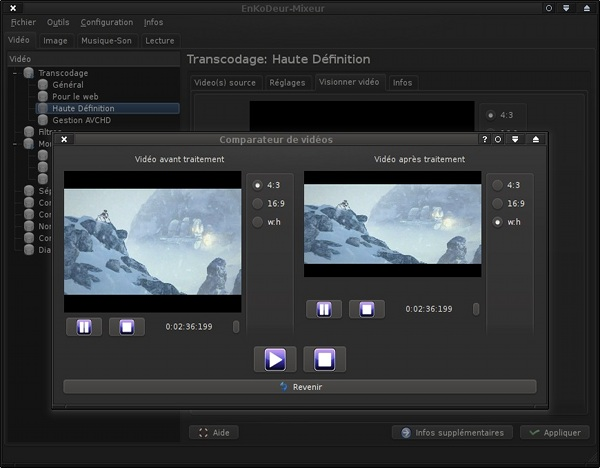
\includegraphics[scale=0.50]{ressources/ekd_linux_redim.jpg}
\end{frame}

\begin{frame}
\frametitle{EKD : Découpage de vidéo}
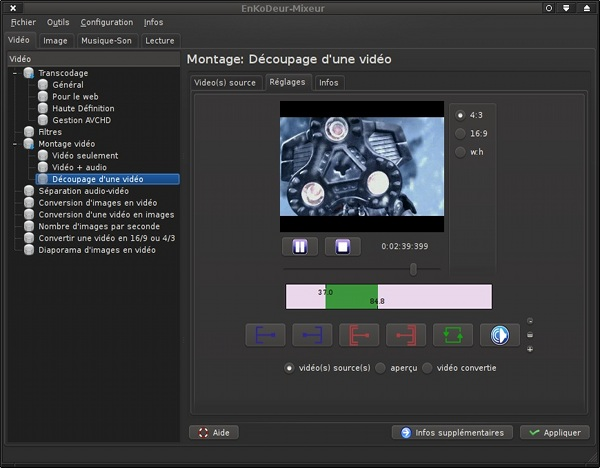
\includegraphics[scale=0.50]{ressources/ekd_linux_decoup.jpg}
\end{frame}

\begin{frame}
\frametitle{EKD : Création de couche alpha}
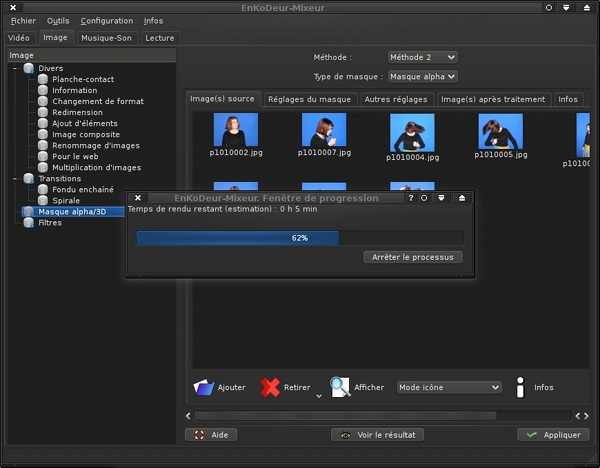
\includegraphics[scale=0.50]{ressources/ekd_linux_alpha1.jpg}
\end{frame}

\begin{frame}
\frametitle{EKD : Création de couche alpha}
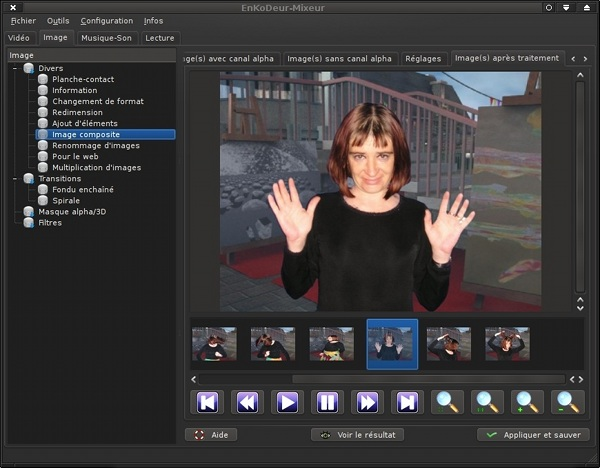
\includegraphics[scale=0.50]{ressources/ekd_linux_alpha2.jpg}
\end{frame}


\begin{frame}
\frametitle{Autoring : Finalisation d'un DVD}
\end{frame}

\begin{frame}
\frametitle{Sources utilisées pour cette présentation}
\href{http://lprod.org/wiki/doku.php/video}{http://lprod.org/wiki/doku.php/video}

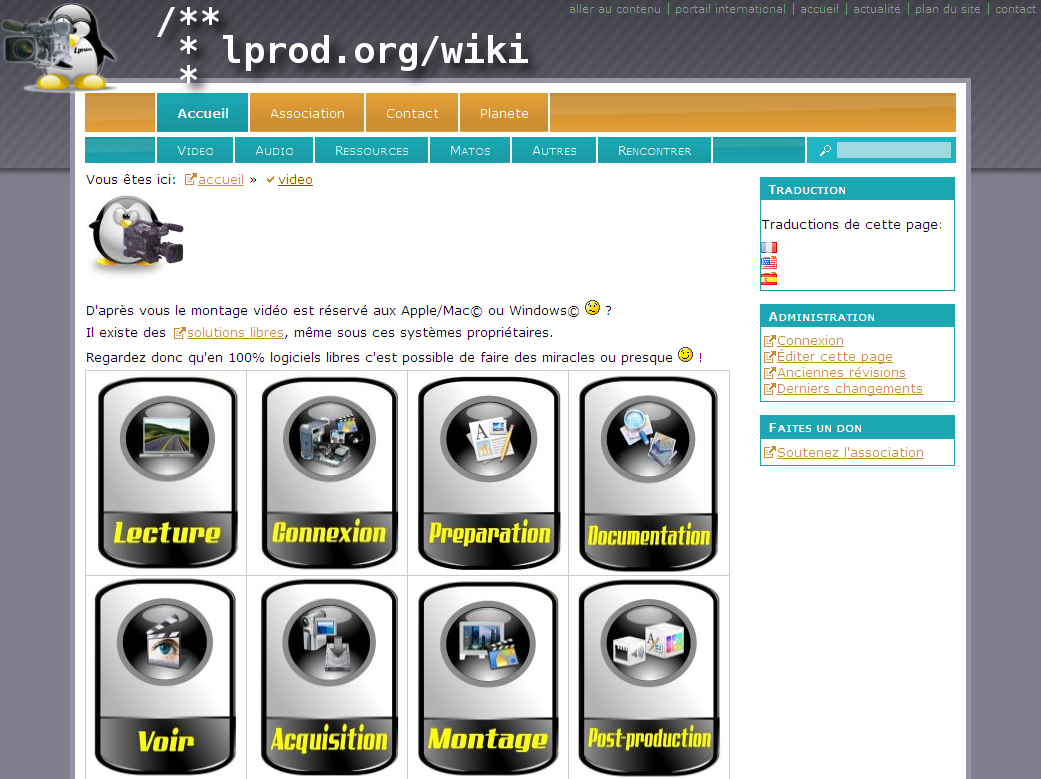
\includegraphics[scale=0.20]{ressources/LPROD.png}

\end{frame}

\end{document}

